\chapter{Appendix}
  \label{sec:appendix}

  \subsection{Figures}

  \begin{figure}[H]
    \centering
    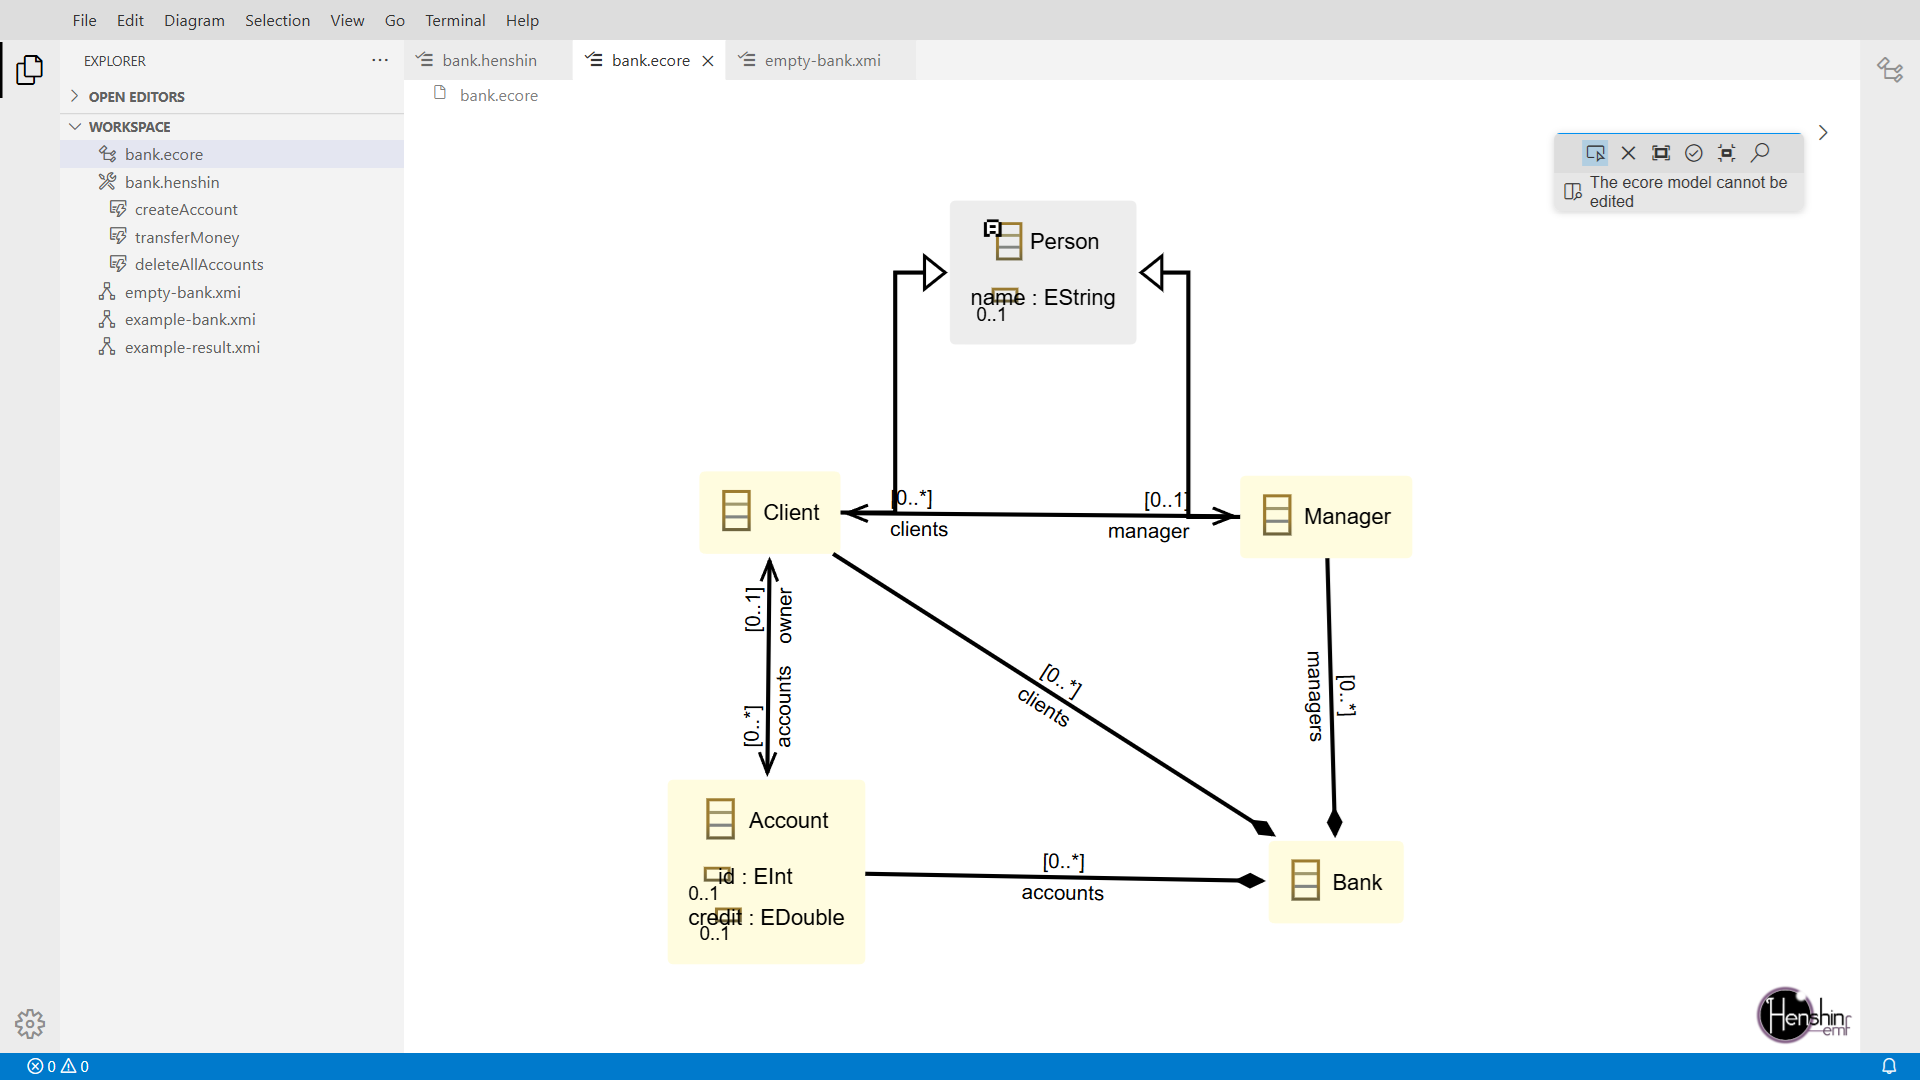
\includegraphics[width=1\textwidth]{ecore-ui}
    \caption{Henshin Web Ecore graph editor}
    \label{fig:ecore-ui}
  \end{figure}

  \begin{figure}[H]
    \centering
    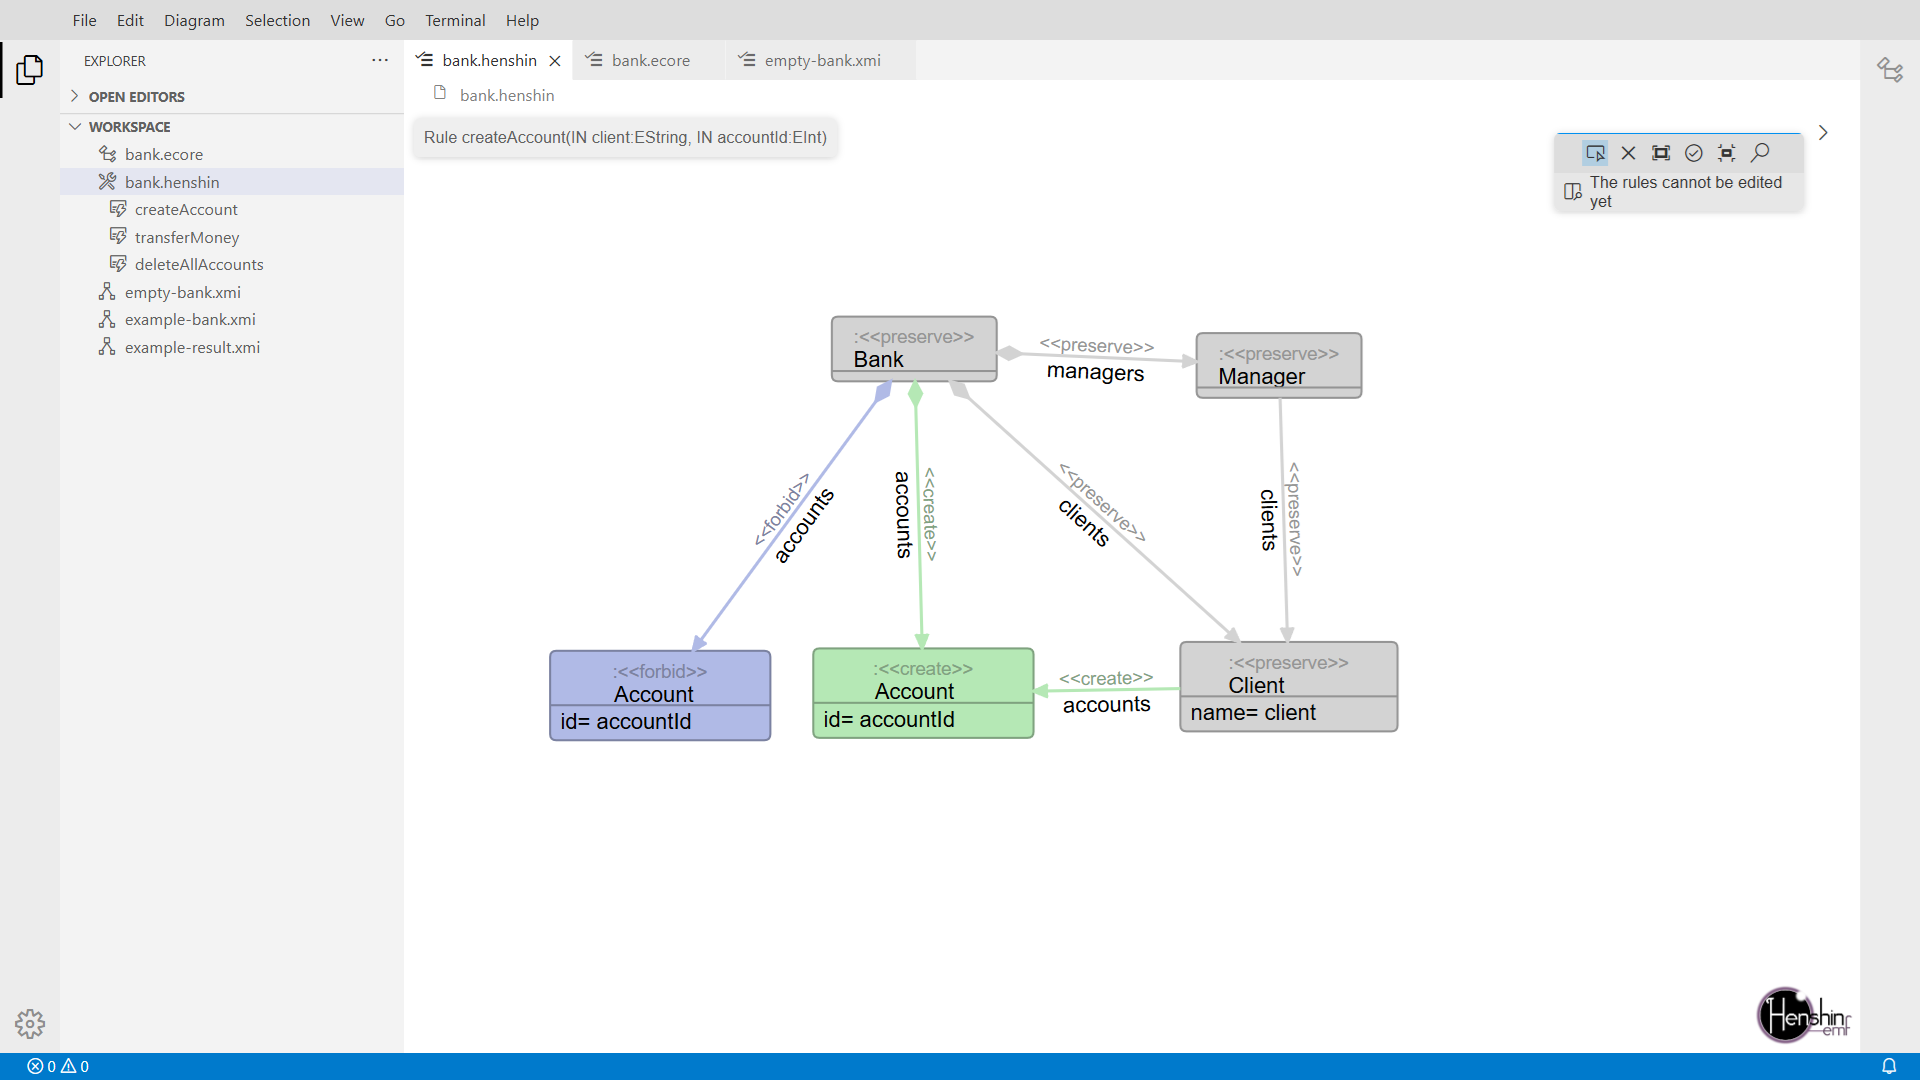
\includegraphics[width=1\textwidth]{rule-ui}
    \caption{Henshin Web Rules graph editor}
    \label{fig:rule-ui}
  \end{figure}

  \begin{figure}[H]
    \centering
    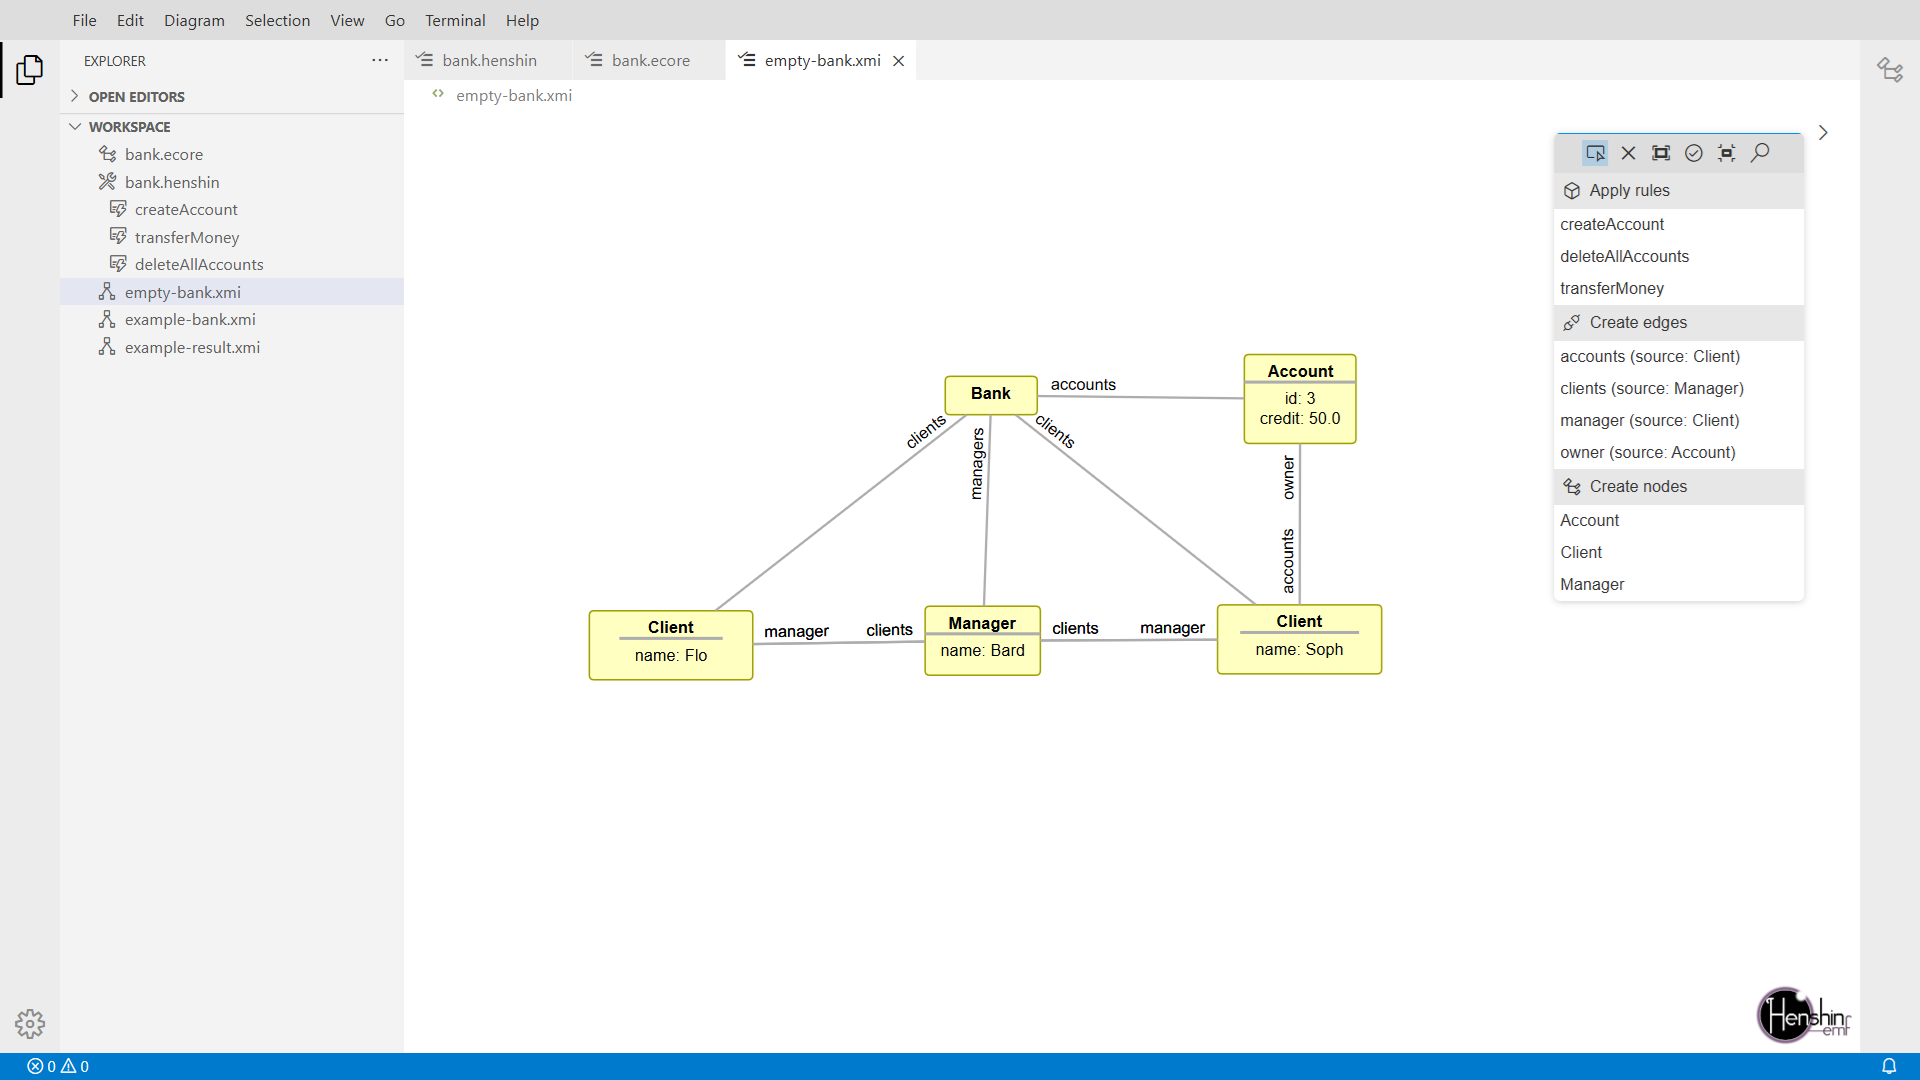
\includegraphics[width=1\textwidth]{xmi-ui}
    \caption{Henshin Web Instance graph editor}
    \label{fig:xmi-ui}
  \end{figure}

  % User Guide
  \begin{figure}[h]
    \centering
    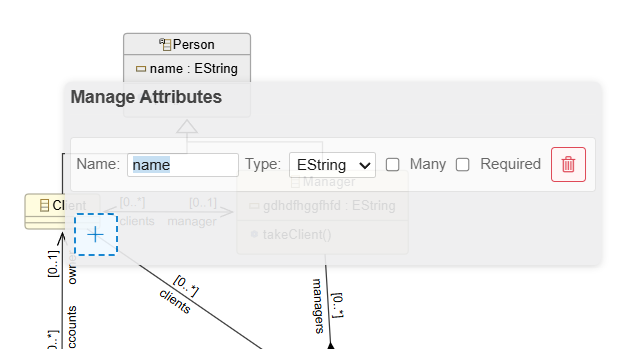
\includegraphics[width=0.7\textwidth]{attribute-editor}
    \caption{Attribute Editor Window}
    \label{fig:attribute-editor}
  \end{figure}
  \begin{figure}[h]
    \centering
    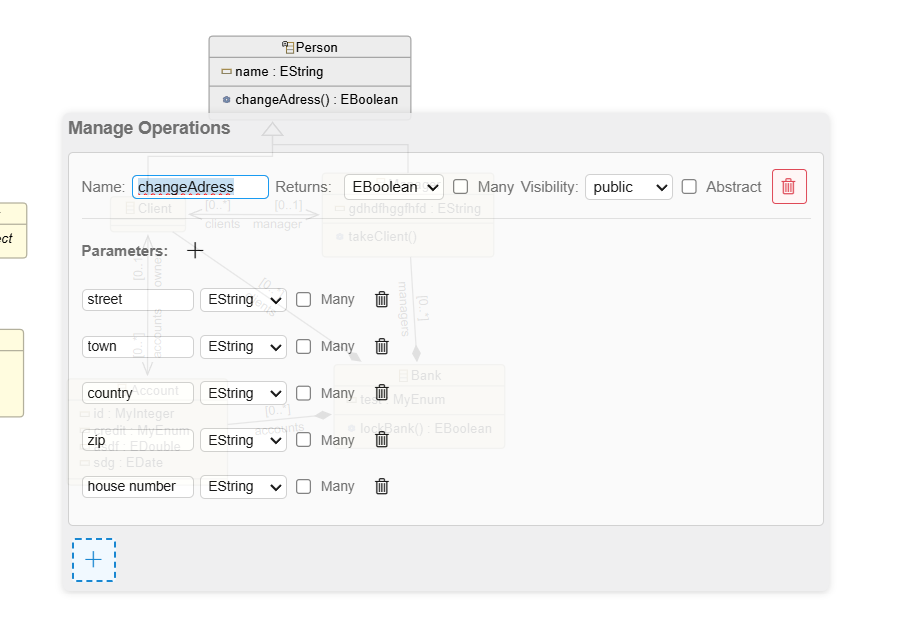
\includegraphics[width=0.7\textwidth]{operation-editor}
    \caption{Operation Editor Window}
    \label{fig:operation-editor}
  \end{figure}
  \begin{figure}[h]
    \centering
    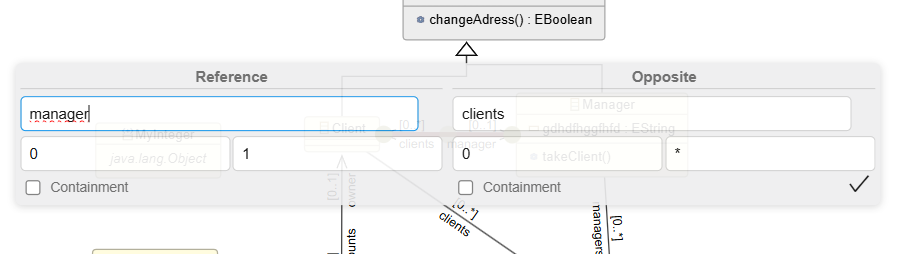
\includegraphics[width=0.7\textwidth]{reference-editor}
    \caption{Reference Editor Window}
    \label{fig:reference-editor}
  \end{figure}
  \begin{figure}[h]
    \centering
    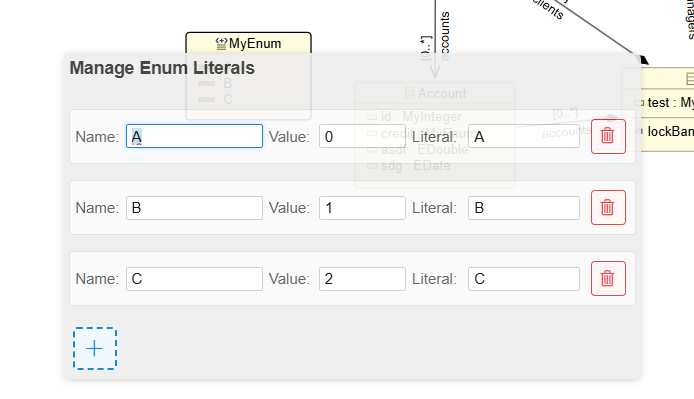
\includegraphics[width=0.7\textwidth]{enum-editor}
    \caption{Enum Editor Window}
    \label{fig:enum-editor}
  \end{figure}
    \begin{figure}[h]
    \centering
    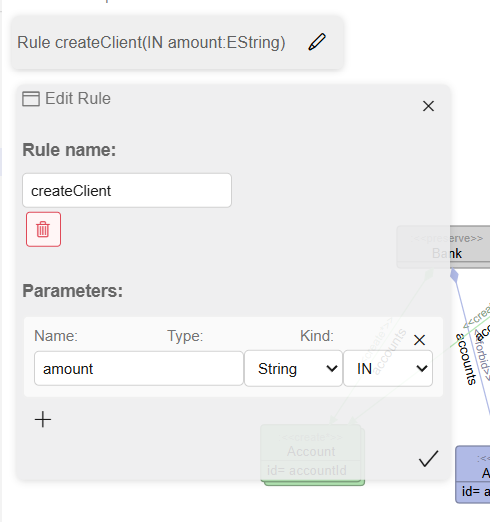
\includegraphics[width=0.7\textwidth]{rule-editor}
    \caption{Rule Editor Window}
    \label{fig:rule-editor}
  \end{figure}

  \subsection{Code Listings}

    % \begin{lstlisting}[language=Java, caption={Parts of \code{NotationAdapter}}, label={lst:notation-adapter}]
public class NotationAdapter extends AdapterImpl {
    private Shape shape;

    public NotationAdapter(Shape shape) {
        this.shape = shape;
    }

    @Override
    public boolean isAdapterForType(Object type) {
        return type == NotationAdapter.class;
    }

    public static Shape getOrAssignNotation(DynamicEObjectImpl obj) {
        // Return existing Notation if present
        for (var adapter : obj.eAdapters()) {
            if (adapter instanceof NotationAdapter) {
                return ((NotationAdapter) adapter).getShape();
            }
        }

        // Assign new Notation
        String hashId = hashENodeObject(obj);
        Shape shape = notationMap.get(hashId);
        if(shape == null) {
            shape = XMINotationFactory.createNewShape(obj);
        }
        NotationAdapter newAdapter = new NotationAdapter(shape);
        obj.eAdapters().add(newAdapter);

        return shape;
    }

    public static String hashENodeObject(DynamicEObjectImpl eObject) {
        StringBuilder result = new StringBuilder();

        result.append(eObject.eClass().getName()).append(":");
        result.append(DynamicEObjectImpl.class.getSimpleName());

        for (EStructuralFeature feature : eObject.eClass().getEAllStructuralFeatures()) {
            if (feature instanceof EAttribute) {
                result.append("-").append(feature.getName());
                result.append(":").append(feature.getEType().getName());
                result.append("=").append(eObject.eGet(feature).toString());
            }
        }

        return result.toString();
    }

    public static void dispose() {
        notationMap.clear();
    }
}
\end{lstlisting}

    % \begin{lstlisting}[language=Java, caption={Parts of \code{XMIGModelFactory}}, label={lst:gmodel-factory}]
@Override
protected void fillRootElement(GModelRoot newRoot) {
    EGraph instanceNodes = modelState.getInstanceGraph();

    newRoot.getChildren().addAll(instanceNodes.stream()
            .map(eObject -> (DynamicEObjectImpl) eObject) //
            .map(this::createNode)//
            .toList());

    ...
}

public GNode createNode(DynamicEObjectImpl eObject) {
    String type = DefaultTypes.NODE;
    if(eObject.eContainer() == null) {
        type = HenshinTypes.XMI_ROOT_NODE;
    }

    GNodeBuilder b = new GNodeBuilder(type) //
            .id(UUIDAdapter.getOrAssignId(eObject)) //
            .layout(GConstants.Layout.VBOX) //
            .addCssClass(HenshinCss.XMI_NODE) //
            .addArguments(GArguments.cornerRadius(3))
            .add(buildHeader(eObject));
    if(!eObject.eClass().getEAllAttributes().isEmpty()) {
        b.add(createAttributesCompartment(eObject.eClass().getEAllAttributes(), eObject));
    }
    applyShapeData(eObject,b);
    return b.build();
}

private GLabel buildHeader(EObject eObject) {
    return new GLabelBuilder(DefaultTypes.LABEL) //
            .id(UUIDAdapter.toLabelId(eObject))
            .addCssClass(HenshinCss.XMI_LABEL)
            .text(eObject.eClass().getName()) //
            .build();
}

...
\end{lstlisting}

